\documentclass{article}

\usepackage{fancyhdr}
\usepackage{hyperref}
\usepackage{graphicx}

\hypersetup{
    colorlinks=true,
    linkcolor=blue,
    filecolor=magenta,      
    urlcolor=blue,
    pdftitle={Day 2},
    pdfpagemode=FullScreen,
    pdfauthor={Taraash},
}

\pagestyle{fancy}
\fancyhead[R]{Week 1 notes}
\fancyfoot[L]{IGDA IIIT-D}
\fancyfoot[C]{\thepage}
\renewcommand{\headrulewidth}{0pt}

\title{Week 1 Recap}
\author{Taraash}
\date{}

\begin{document}
\maketitle

\tableofcontents
\newpage

This is in continuation of the Day 1 notes, which you can find \href{https://drive.google.com/file/d/1gTv4I6fxLQCYuvl5RoD4AZJ5WyXFFGp4/view?usp=sharing}{here}. (These notes cover more information than what I talked about in the class, so if you attended the class, you should still read these.)

\section{Materials}
A material is a collection of properties or parameters that define how an object interacts with light and other objects in a 3D environment.

A non-exhaustive list of properties that can be defined in a material includes:
\begin{itemize}
    \item Diffuse Color
    \item Roughness
    \item Metallic
    \item Transparency
    \item Emissive Color
    \item Normal Map
\end{itemize}

For example, this is Blender's Principled BSDF shader, which is a physically based shader that combines multiple properties into one node:

\begin{figure}[h]
    \centering
    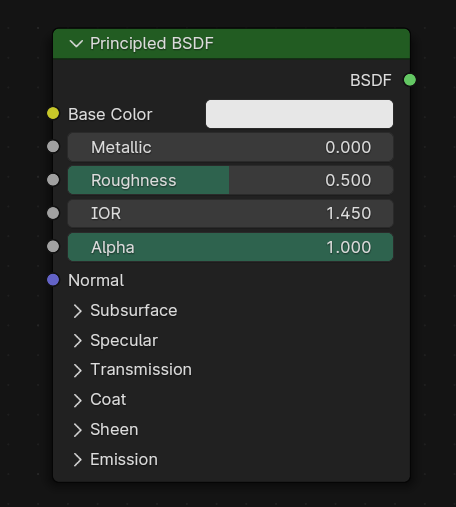
\includegraphics[width=0.6\textwidth]{day2images/image.png}
    \caption{Blender's Principled BSDF Shader}
    \label{fig:principled_bsdf}
\end{figure}

The fun part is instead of using a single value as being the same everywhere on the object, we can use a texture map to define how the property changes across the surface of the object.

\subsection{Texture Maps}
Texture maps are images that define how a material's properties vary across the surface of a 3D object. To understand this we will need to know about UV mapping, which I won't go over in much detail but briefly, UV mapping is the process of projecting a 2D image onto a 3D model's surface. The ``U'' and ``V" refer to the axes of the 2D texture space, as opposed to the ``X", ``Y", and ``Z" axes of the 3D space. You can find a good explanation of UV mapping \href{https://youtu.be/XeBUfMKKZDo?si=PByk-2xxJS7TuU2l}{here}.

There are many texture maps, and they look different, I'll describe the common ones now.

\subsubsection{Diffuse maps}
They define the base color of any object/material. This is how your object will look like under white light. It is also known as Albedo or Diffuse map. 

\begin{figure}[h]
    \centering
    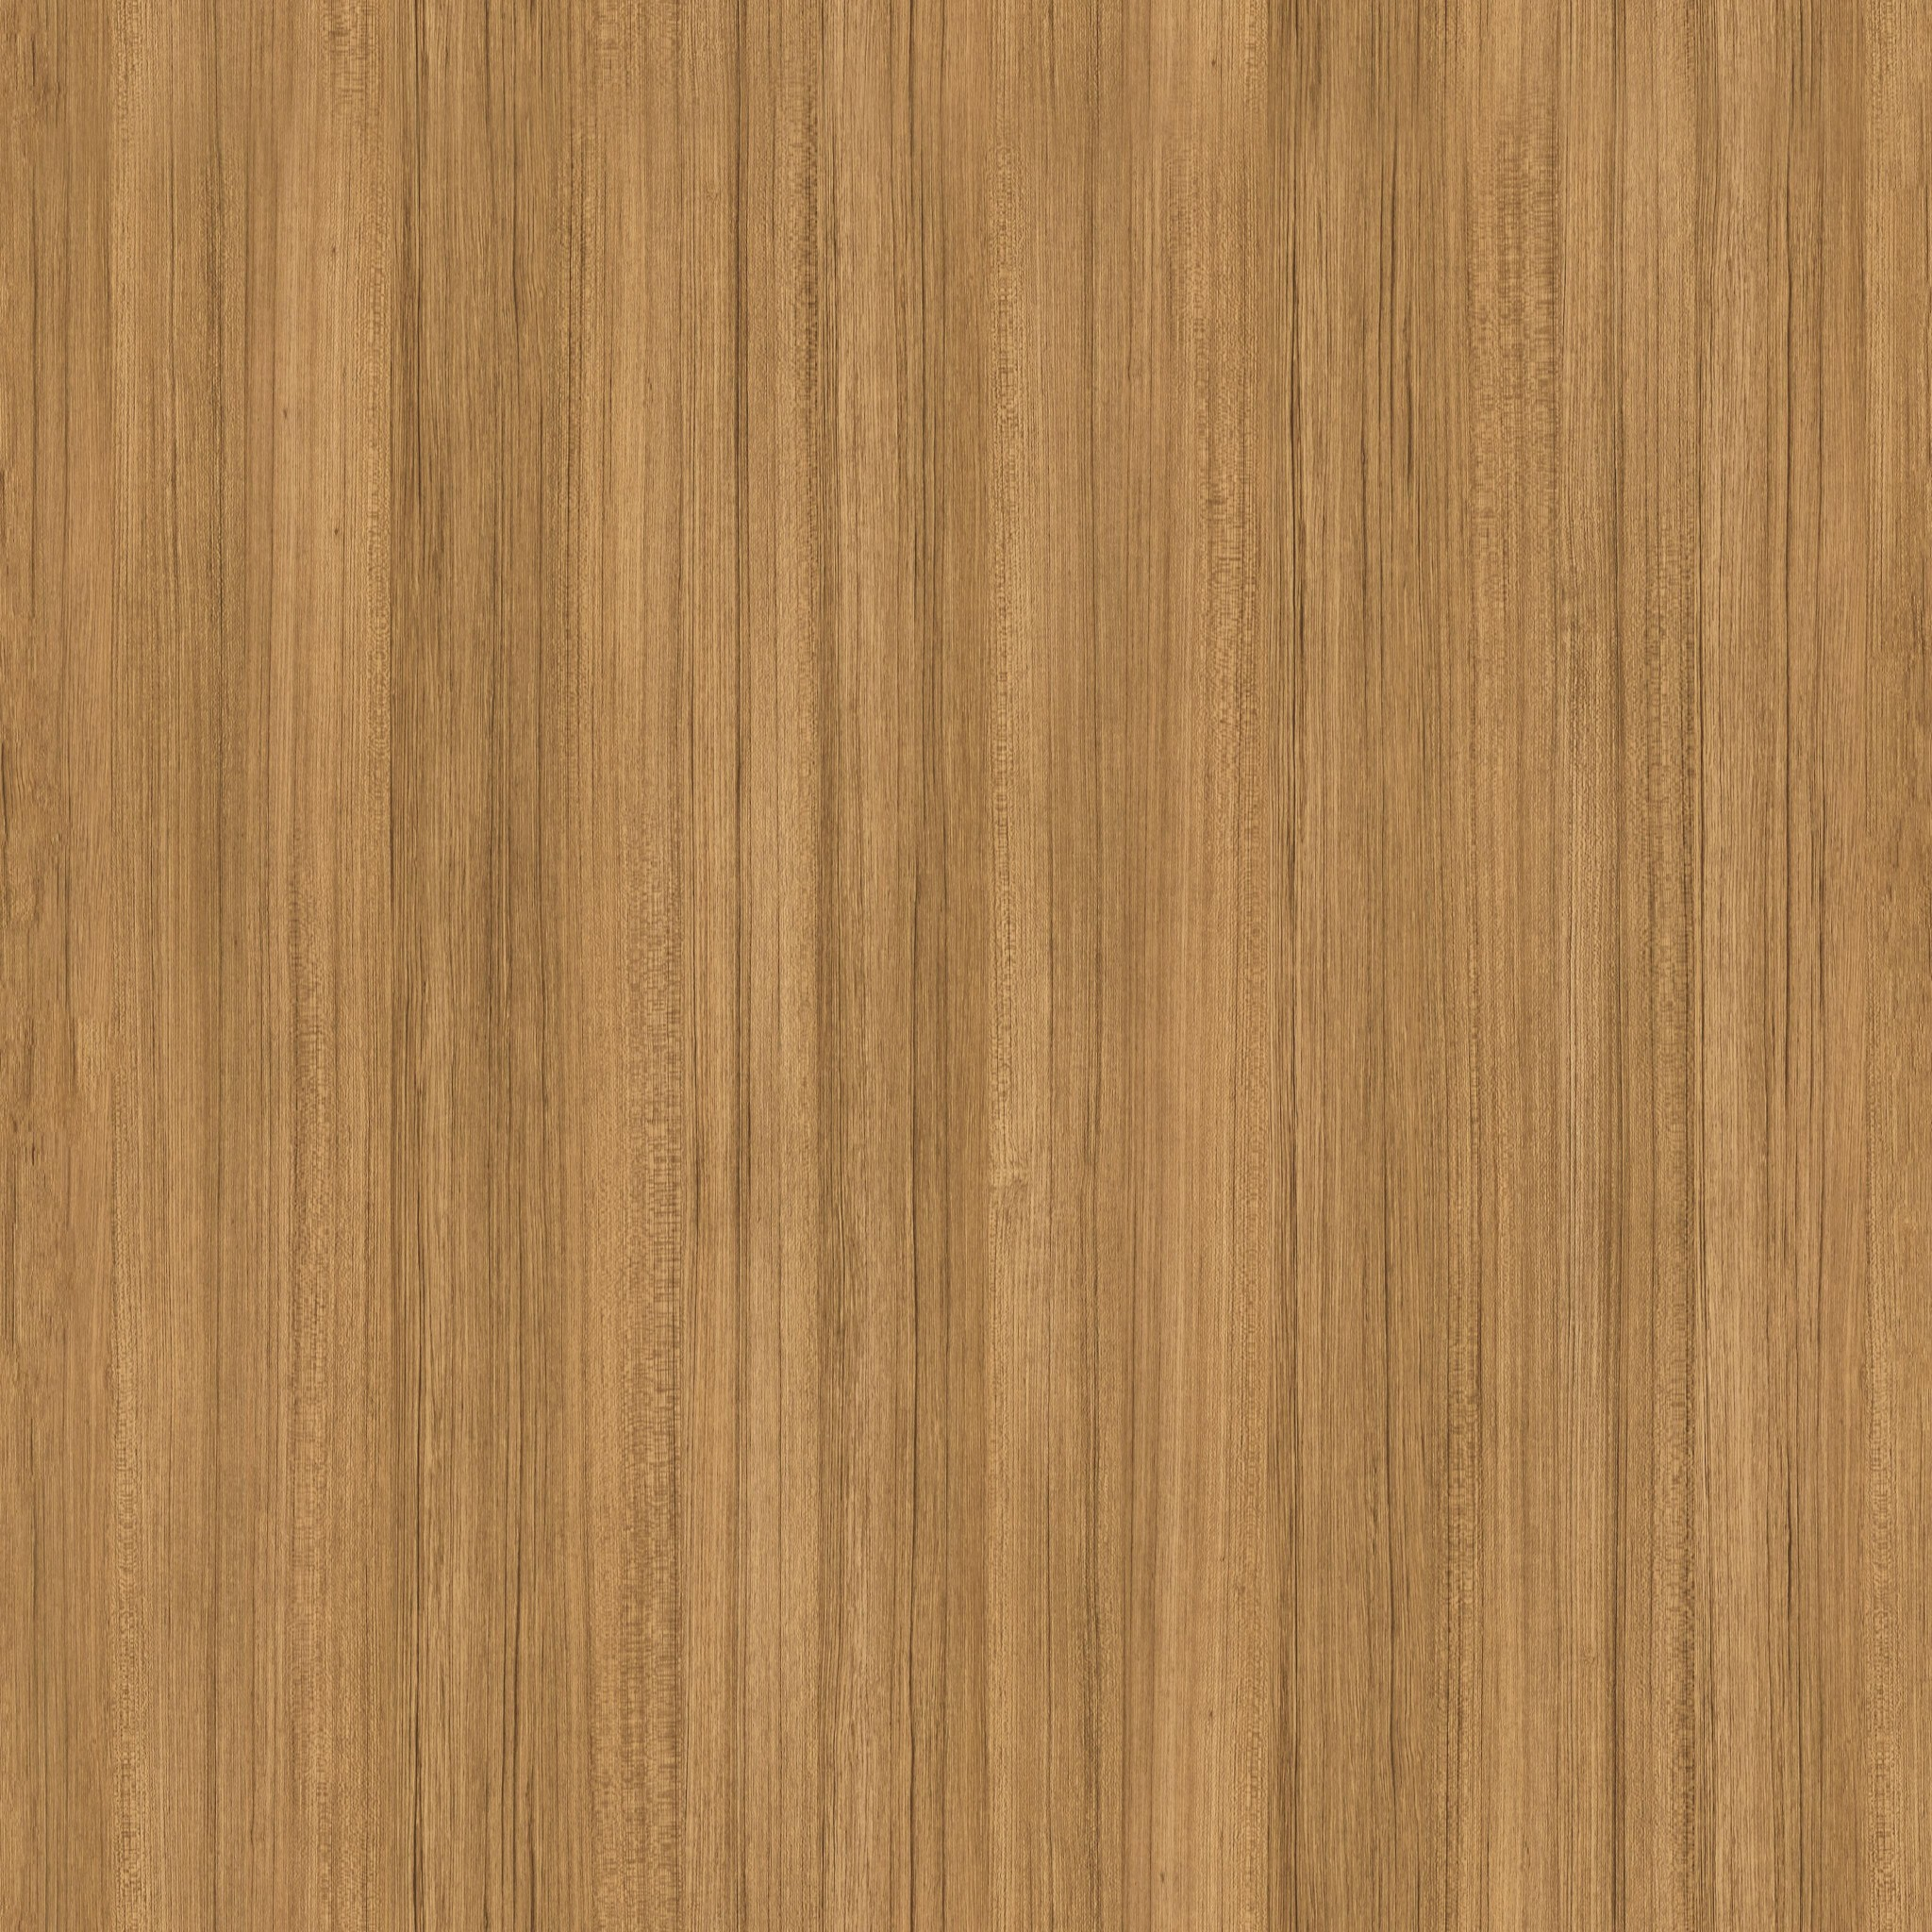
\includegraphics[width=0.6\textwidth]{day2images/Teak_4k_Albedo.jpg}
    \caption{Diffuse map for a Teak wood material}
    \label{fig:diffuse_map}
\end{figure}

\subsubsection{Normal maps}
Normal maps are used to add surface detail without increasing the polygon count of a 3D model. They store information about the surface normals, which affects how light interacts with the surface, creating the illusion of depth and detail. It is important to note that normal maps do not change the actual geometry of the model, they only affect how light interacts with it.
\begin{figure}[h]
    \centering
    
\includegraphics[width=0.6\textwidth]{day2images/Teak_4k_Normal.jpg}
    \caption{Normal map for the Teak wood material}
    \label{fig:normal_map}
\end{figure}
\textit{Zoom far enough into the image to see the details.}

Another thing to note is that normal maps are usually blueish, this is because the RGB values of the normal map correspond to the XYZ coordinates of the surface normals (which are in local space). The blue channel represents the Z-axis (once again, the local Z-axis), which is perpendicular to the surface, while the red and green channels represent the X and Y axes, respectively. There is also usually a little more care to be given to these maps than the Diffuse since they give vector data, but they are still just images. Unreal Engine handles this automatically, but in Blender you need to use a Normal Map node to convert the image data into vector data.

\subsubsection{Roughness maps}
Roughness maps define how rough or smooth a surface is. These are simple black and white images where white represents 1, that is, high roughness. (Some engines use glossy maps instead, which are the inverse of roughness maps, where white represents 0, that is, high glossiness.)

\begin{figure}[!h]
    \centering
    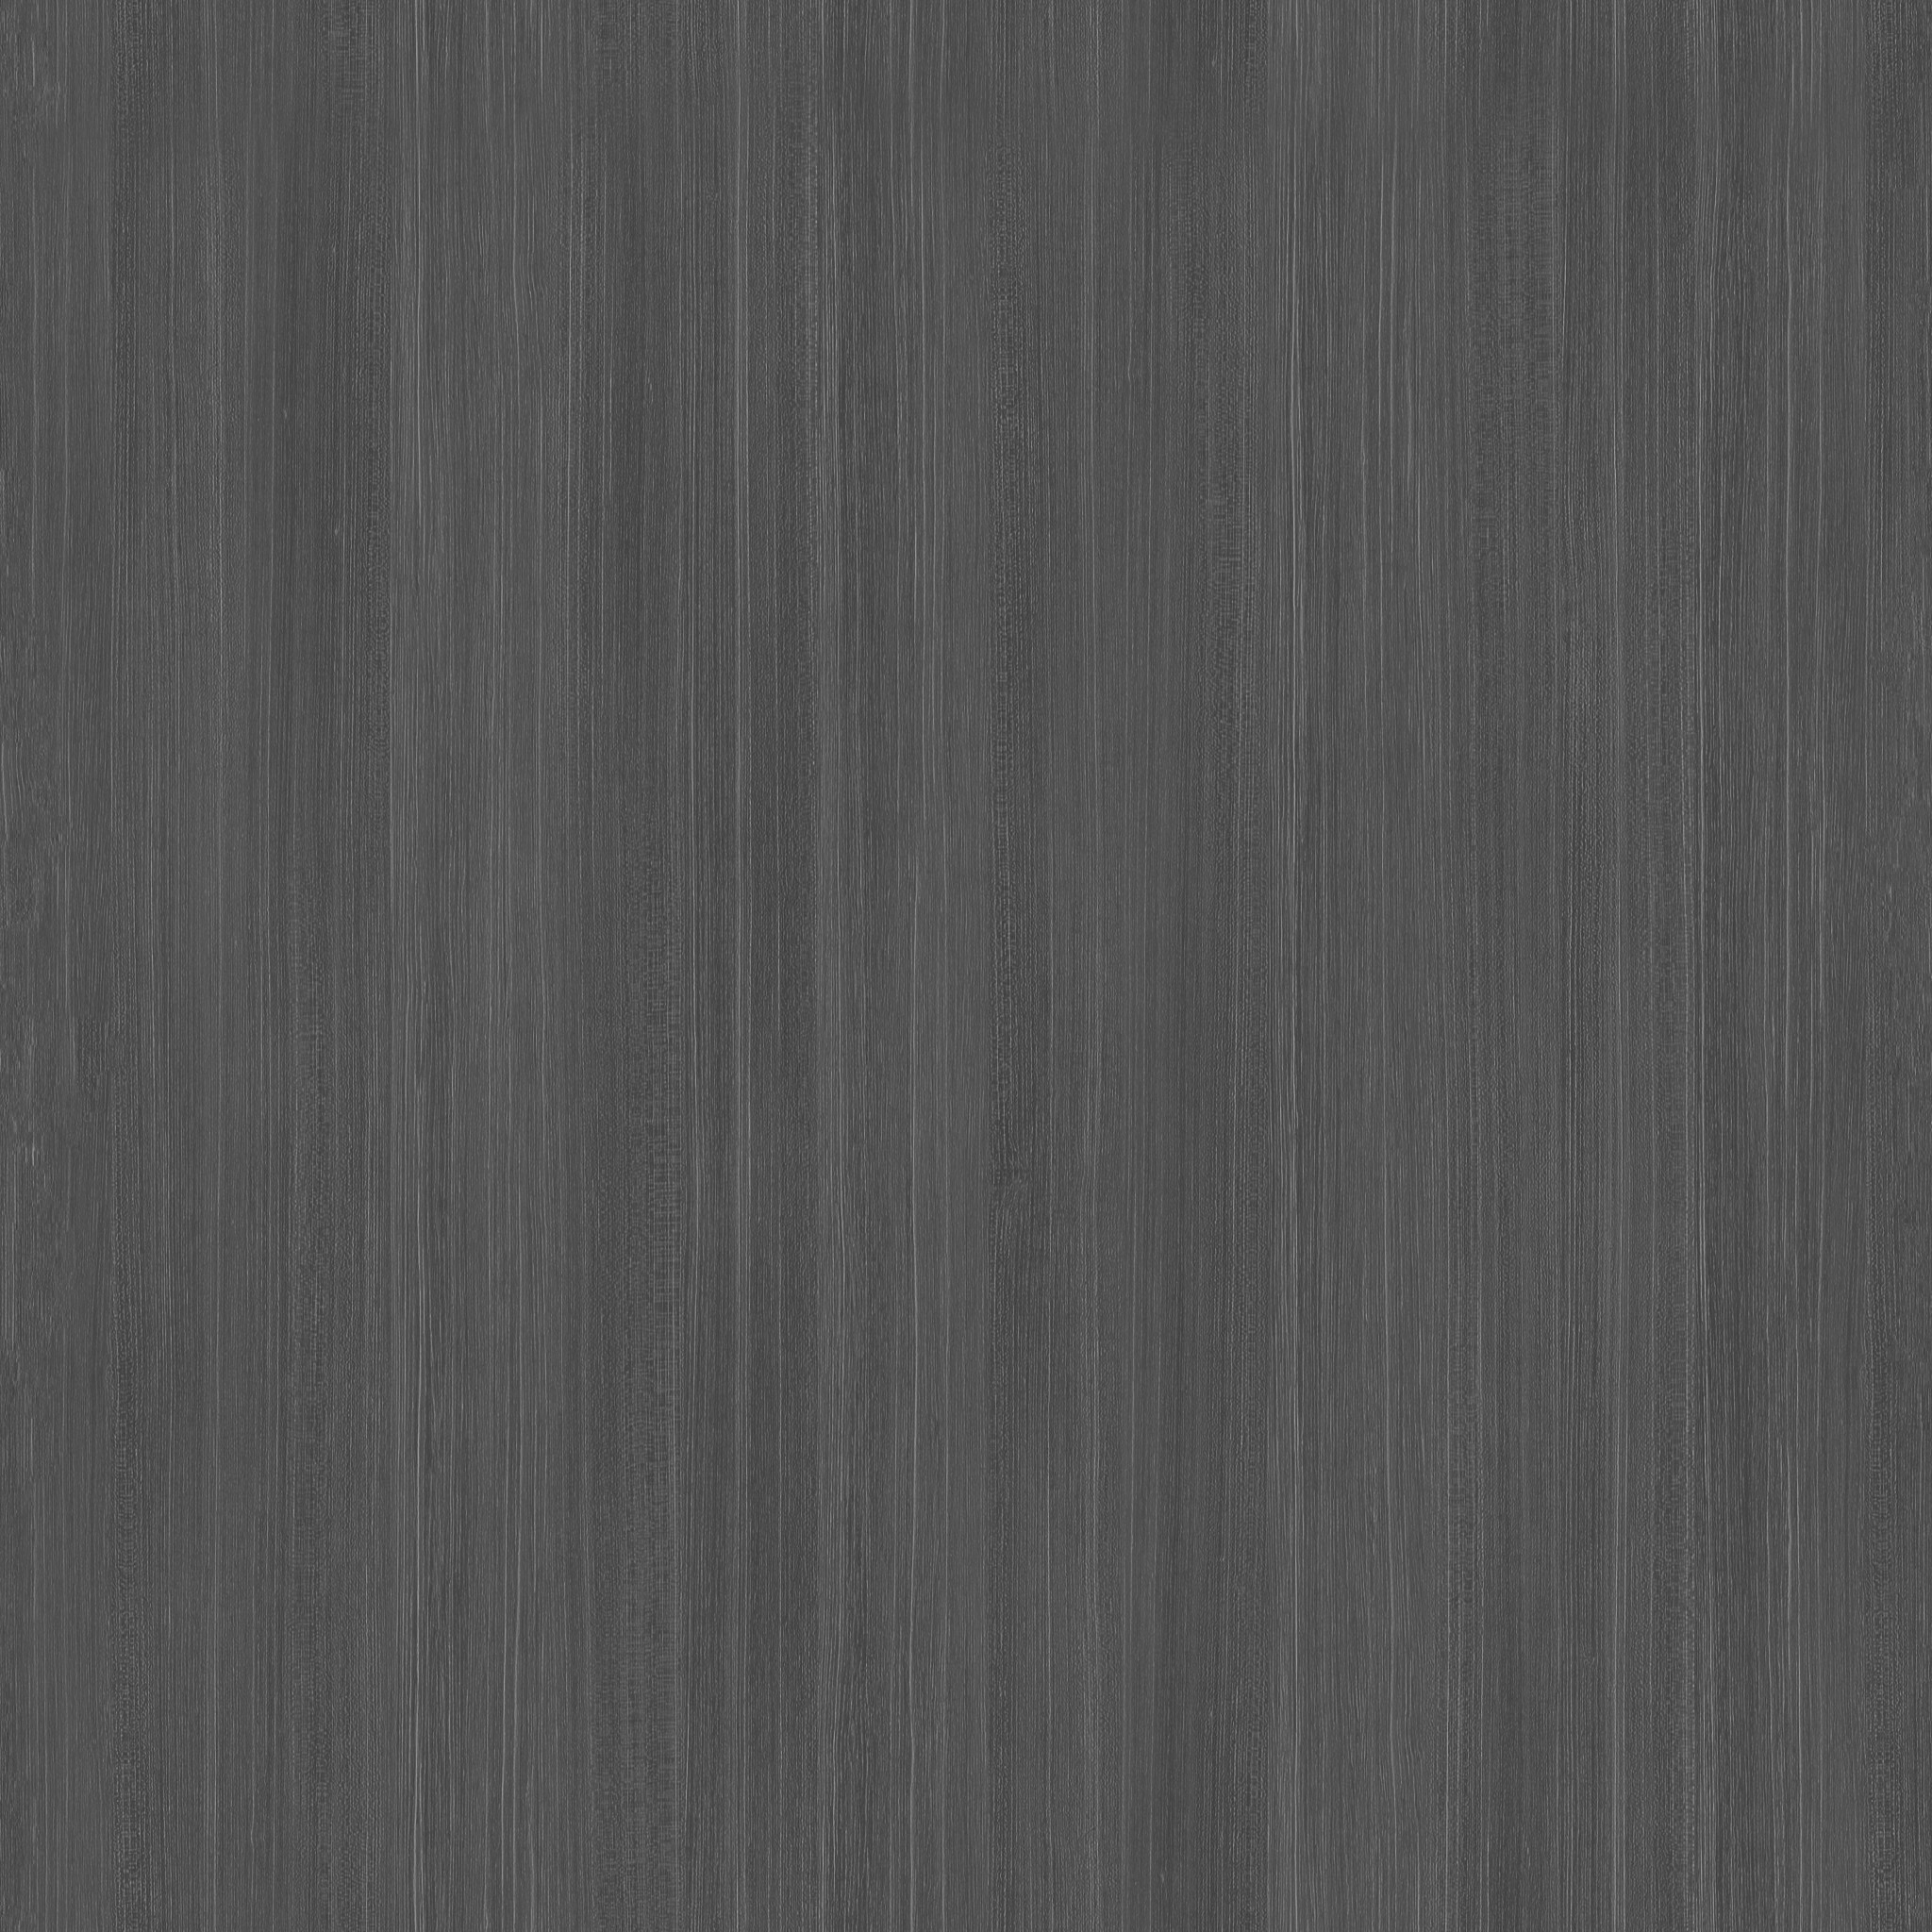
\includegraphics[width=0.6\textwidth]{day2images/Teak_4k_Roughness.jpg}
    \caption{Roughness map for the Teak wood material}
    \label{fig:roughness_map}
\end{figure}

\newpage

These are the maps I thought were the most important, but there are many more types of texture maps, such as metallic maps, ambient occlusion maps, displacement maps, etc. Take a look at Blender's manual for their Principled BSDF shader (\href{https://docs.blender.org/manual/en/4.0/render/shader_nodes/shader/principled.html#bpy-types-shadernodebsdfprincipled}{here}) for more information.

\subsection{Unreal's Material Editor}
Unreal handles materials slightly differently, it has certain material ``types'' that disables and enables certain properties in the master node, take a look at this screenshot of the Material Editor:

\begin{figure}[h]
    \centering
    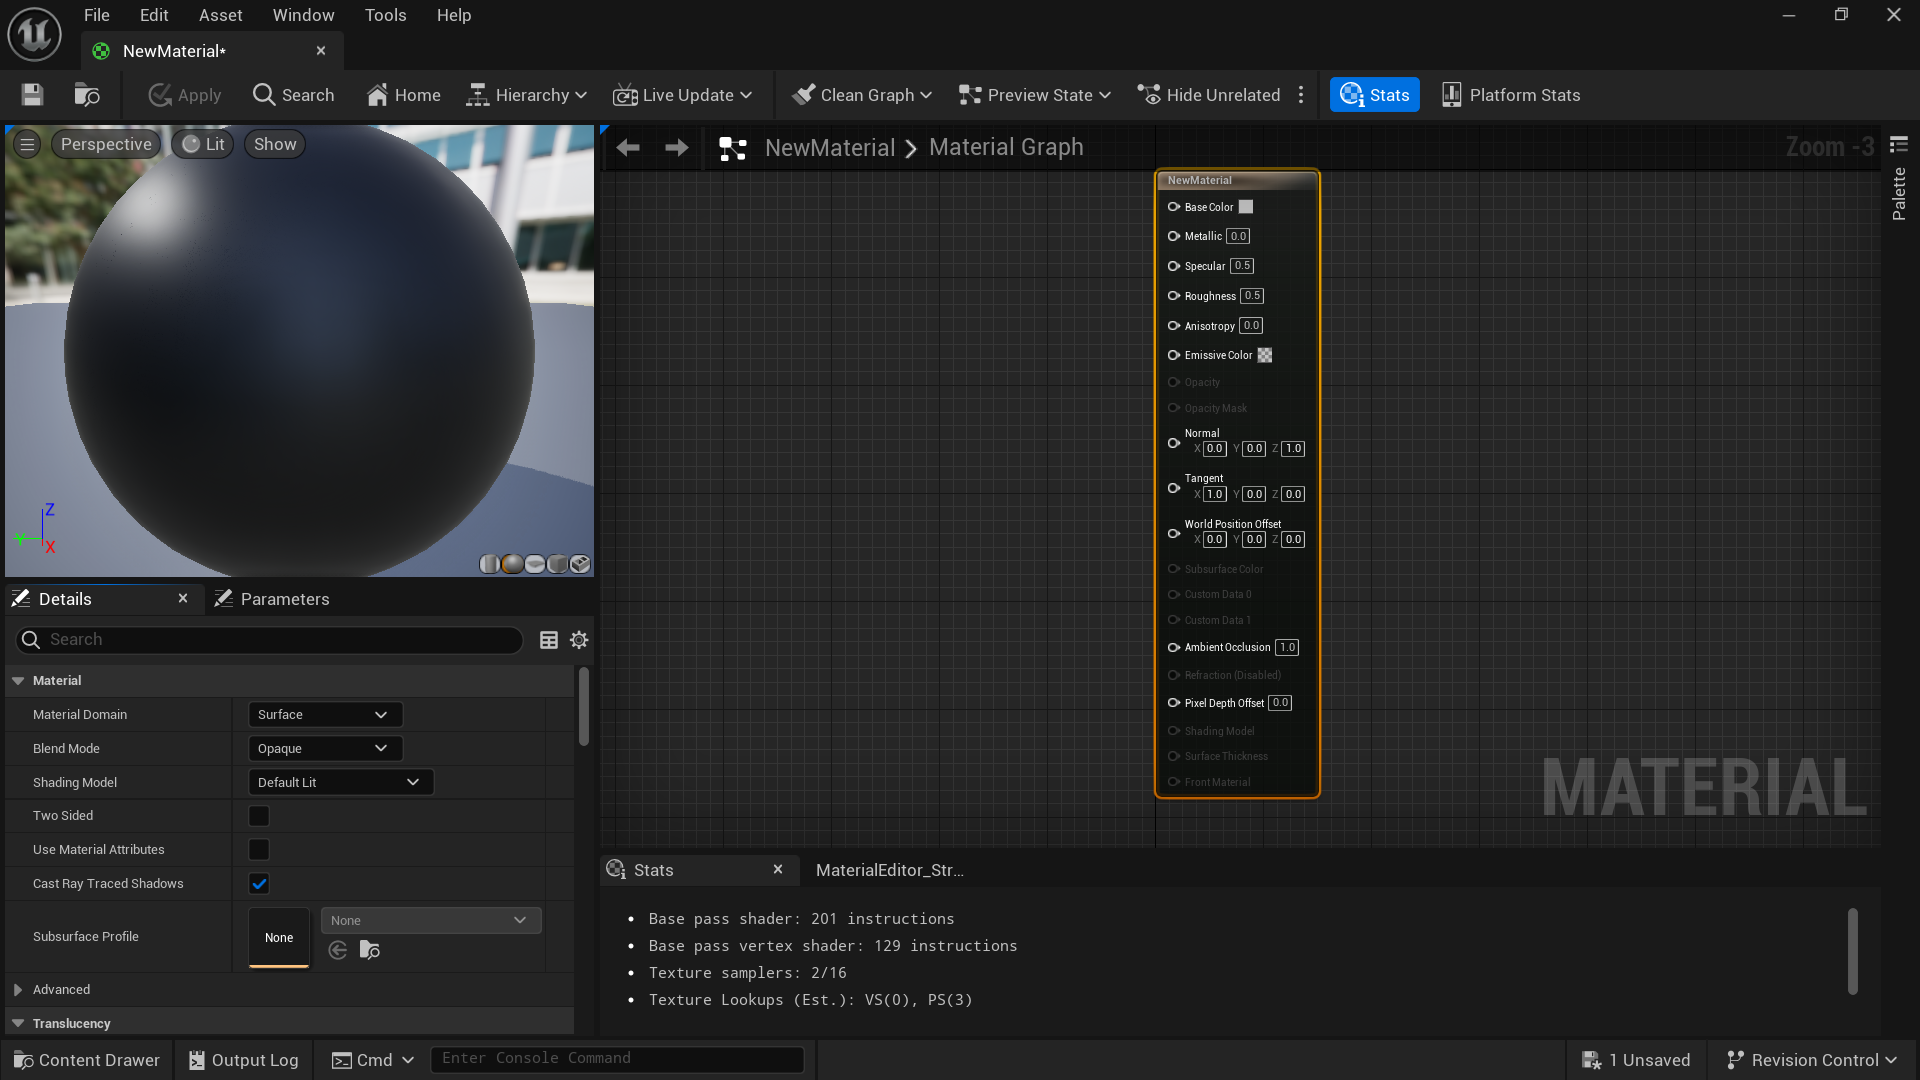
\includegraphics[width=1\textwidth]{day2images/image001.png}
    \caption{Unreal's Material Editor}
    \label{fig:unreal_material_editor}
\end{figure}

\textit{You can get here by right-clicking in the Content Browser and selecting Material. Give it a name and double-click to open it.}

You can immediately find some maps I've talked about before, and you can use the same texture maps here. But there are also some new slots, a notable one is the World Position Offset, which allows you to move the object in the world space. This is useful for creating effects like waving grass or moving water without changing the actual geometry of the object. (In fact, when we'll talk about optimization, we'll talk more about this.)

\subsection{Material Instances}
We didn't talk about this in Day 2, but you can create `variables' or \textit{parameters} in Unreal's Material Editor, which can be used to change the material's properties without having to create a brand-new material. You can create a Material Instance by right-clicking on a material in the Content Browser and selecting Create Material Instance. We'll cover this in Week 2.

\section{Decals}

Decals are a way to project textures onto surfaces in a 3D environment, allowing for additional detail and effects without modifying the underlying geometry. They can be used to create effects like dirt, graffiti, or damage on surfaces. Decals themselves are materials, built with the same maps we've talked about, including an important one we didn't talk about, the \textit{Opacity Mask}. This is a black and white texture that defines which parts of the decal are visible and which are transparent. You place them in the world and rotate it to point or \emph{project} it onto the surface you want to apply it to. (You can uncheck \emph{Receives Decals} on a mesh to prevent it from receiving decals.)

\section{Collision}

We slightly touched upon collisions, when we created a Static Mesh from our brushes we lost the collision we got from the brushes. This meant we could easily walk through the entirety of our mesh and did not respect the boundaries. To specify which parts of the mesh our player should not be able to walk through, we use a \textit{collision mesh}. This is a simplified version of the mesh that defines the boundaries of the object. (You can use the actual mesh as the collision mesh, but it is not recommended for performance reasons, you do this by setting Collision Complexity to ``Use complex collision as simple".) Take a look at this screenshot:

\begin{figure}[h]
    \centering
    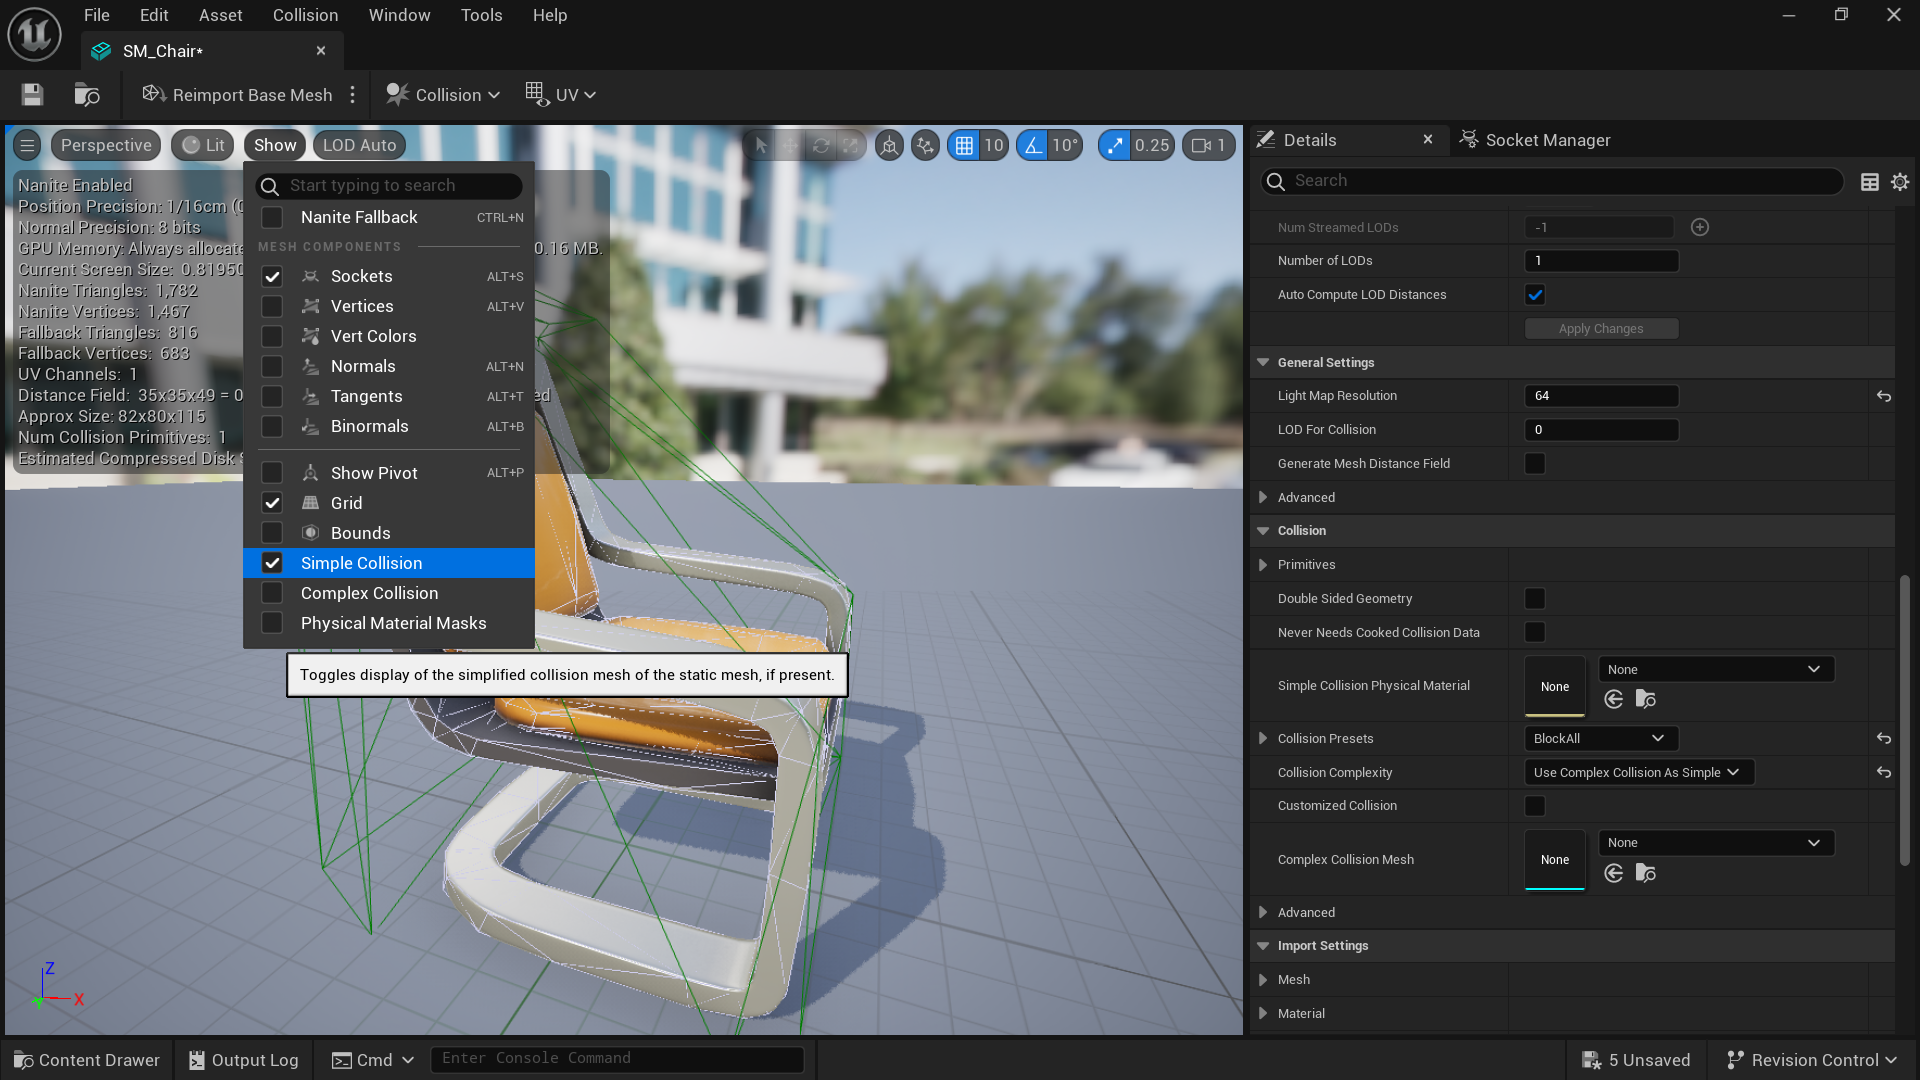
\includegraphics[width=1\textwidth]{day2images/image003.png}
    \caption{Unreal's Static Mesh Editor showing the collision mesh}
    \label{fig:unreal_static_mesh_editor}
\end{figure}

The mesh created by the green edges is the simple collision mesh, usually a convex hull (to visualize these better, I may recommend going to Blender's geometry nodes and using the Convex Hull node, but won't describe that here). The light-purple edges form the complex collision mesh, this gives the highest quality collision but is also the most expensive in terms of performance. (You see these collision meshes by turning them on in the \emph{show} menu on the top left.)

As per our simple building example, we used a few simple boxes to define our collision mesh. You create these by going to the \emph{Collision} button on the top left and selecting \emph{Add box simplified collision}. I recommend you try out the many other options available.

\begin{figure}[h]
    \centering
    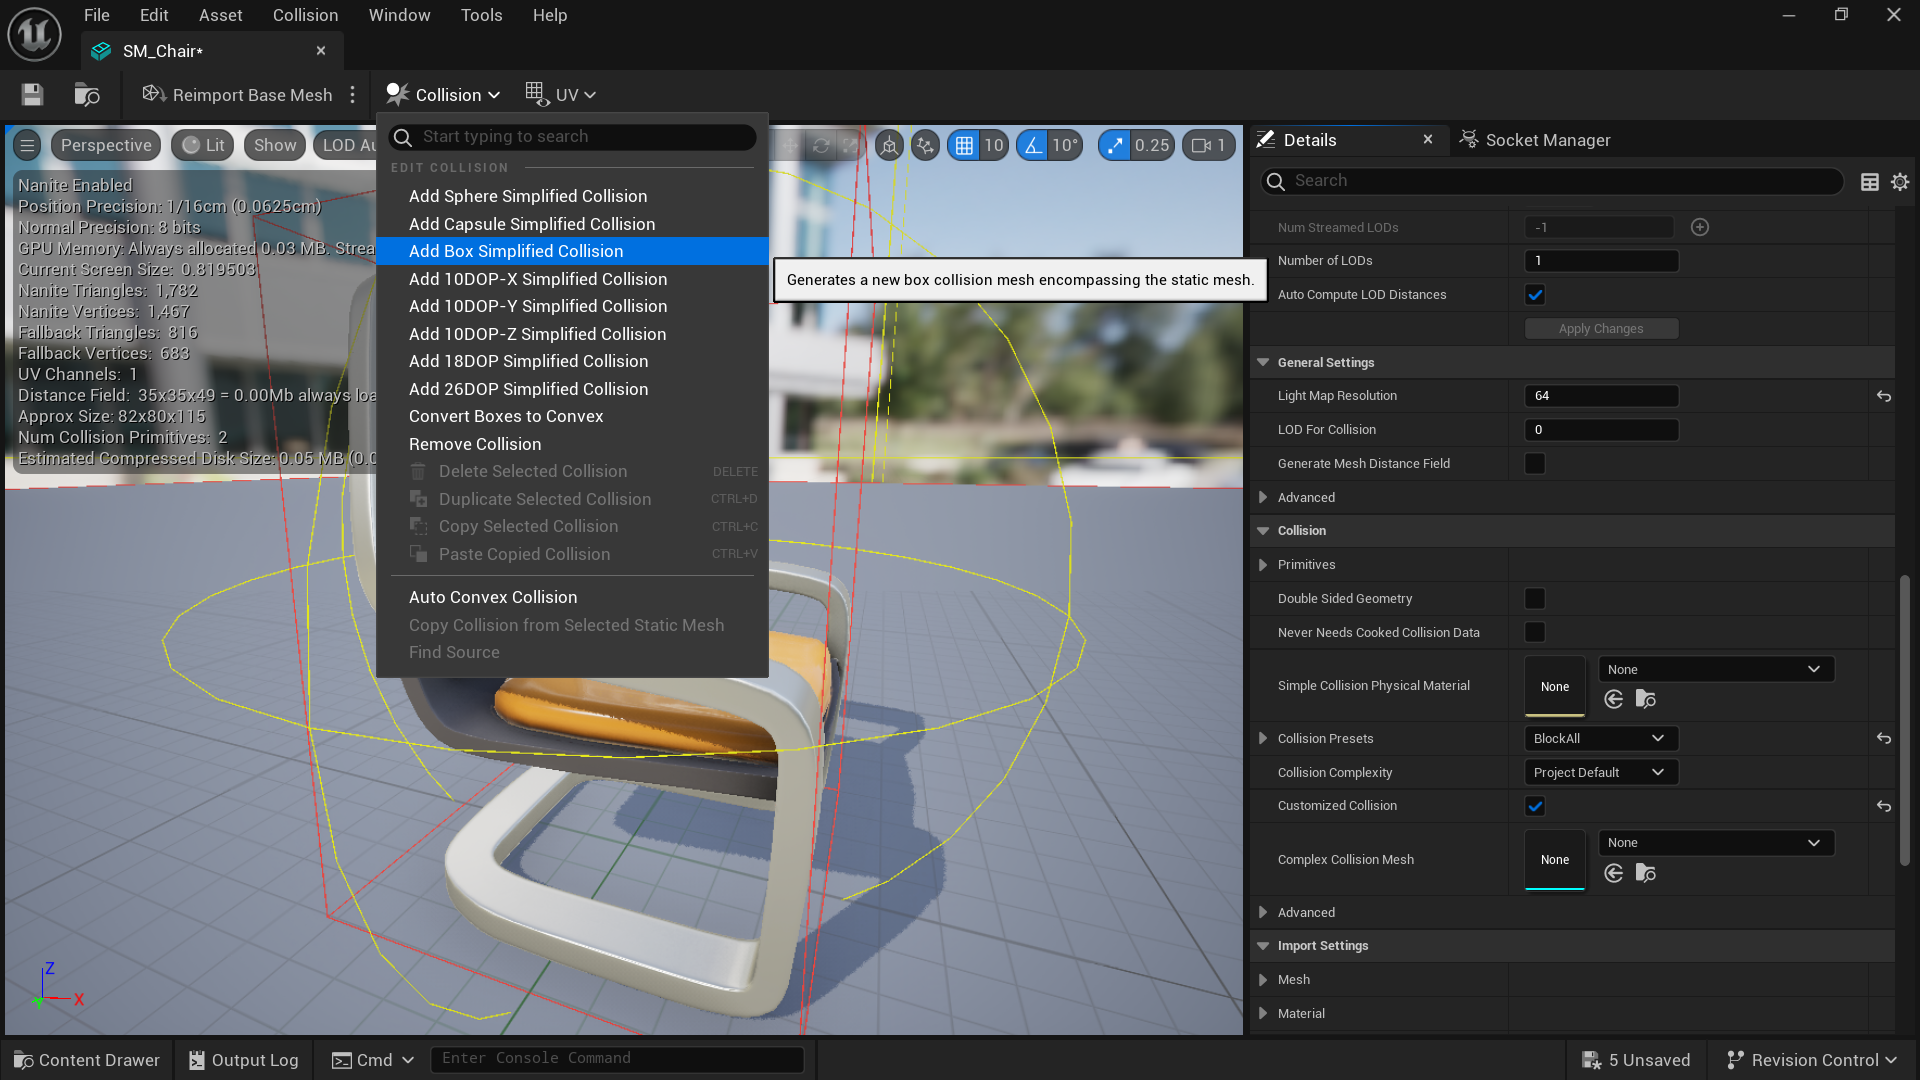
\includegraphics[width=1\textwidth]{day2images/image004.png}
    \caption{Unreal's Static Mesh Editor showing the collision options}
    \label{fig:unreal_collision_options}
\end{figure}

\newpage

We can now scale this new box we obtained by our usual gizmos (remember, \emph{space} cycles between them). We can add many such cubes to specify the collision mesh, and you'll often find you end up with a less dense mesh than the complex collision mesh with the same quality.
\\[10pt]
This is pretty much all the stuff we covered in Week 1, I'll now address some doubts I received.

\section{Foliage}

Foliage is collectively used to refer grass, flowers, tress, rocks and other natural elements like fallen sticks, leaves, etc. It's very easy to use and paint foliage over your landscape. Simply download a pack you like (I recommend the \href{https://fab.com/s/f294bc8824ff}{temperate vegetaion} packs, there are many of them, and all are free!). After downloading, open the folder in the content browser, navigate to the \emph{foliage} folder, and drag the foliage you like to where it says `+ Drop Foliage Here' (you need to be in the foliage mode here, the previous doc has an image). Simply check the foliage you want to paint, make sure you're using the paint brush, and paint in your foliage on the landscape. (You can paint foliage over static meshes, brushes, and other foliage as well! Take a look at the \emph{Filters} section.)
That's pretty much it, you can change the normal brush settings, and could also click on a foliage asset and change its individual settings that show up below it.

\section{Brushes}
A quick bit about brushes. They very easily allow us to create materials and boolean operations, to carve out windows and doors and other shapes. But they do not accurately reflect light, which is why we must convert them to a static mesh. You must select every brush that is participating in the creation of your building (including selecting the brushes that carve out windows and doors from your final building) and then head on over to \emph{Brush Settings} in the Details pane, twirl down the \emph{Advanced} section and hit `Convert to Static Mesh'. It'll prompt you to save it somewhere, since we just created a new asset, and then you can use it like any other static mesh. That's it.
(By default, brushes would be filled, imagine a solid block of wood, but we can make them hollow by checking the \emph{Hollow} checkbox in the Details pane. This gives our brushes a thickness, and an interior which we can access through our doors or whatever we carve out.)

\section{Running on a slower computer}
If you're having trouble following along because of a slow computer, try these things:
\begin{description}
    \item[Lower your scalability] If you don't see it directly go to Settings \textgreater\, Engine Scalability Settings. \\[10pt]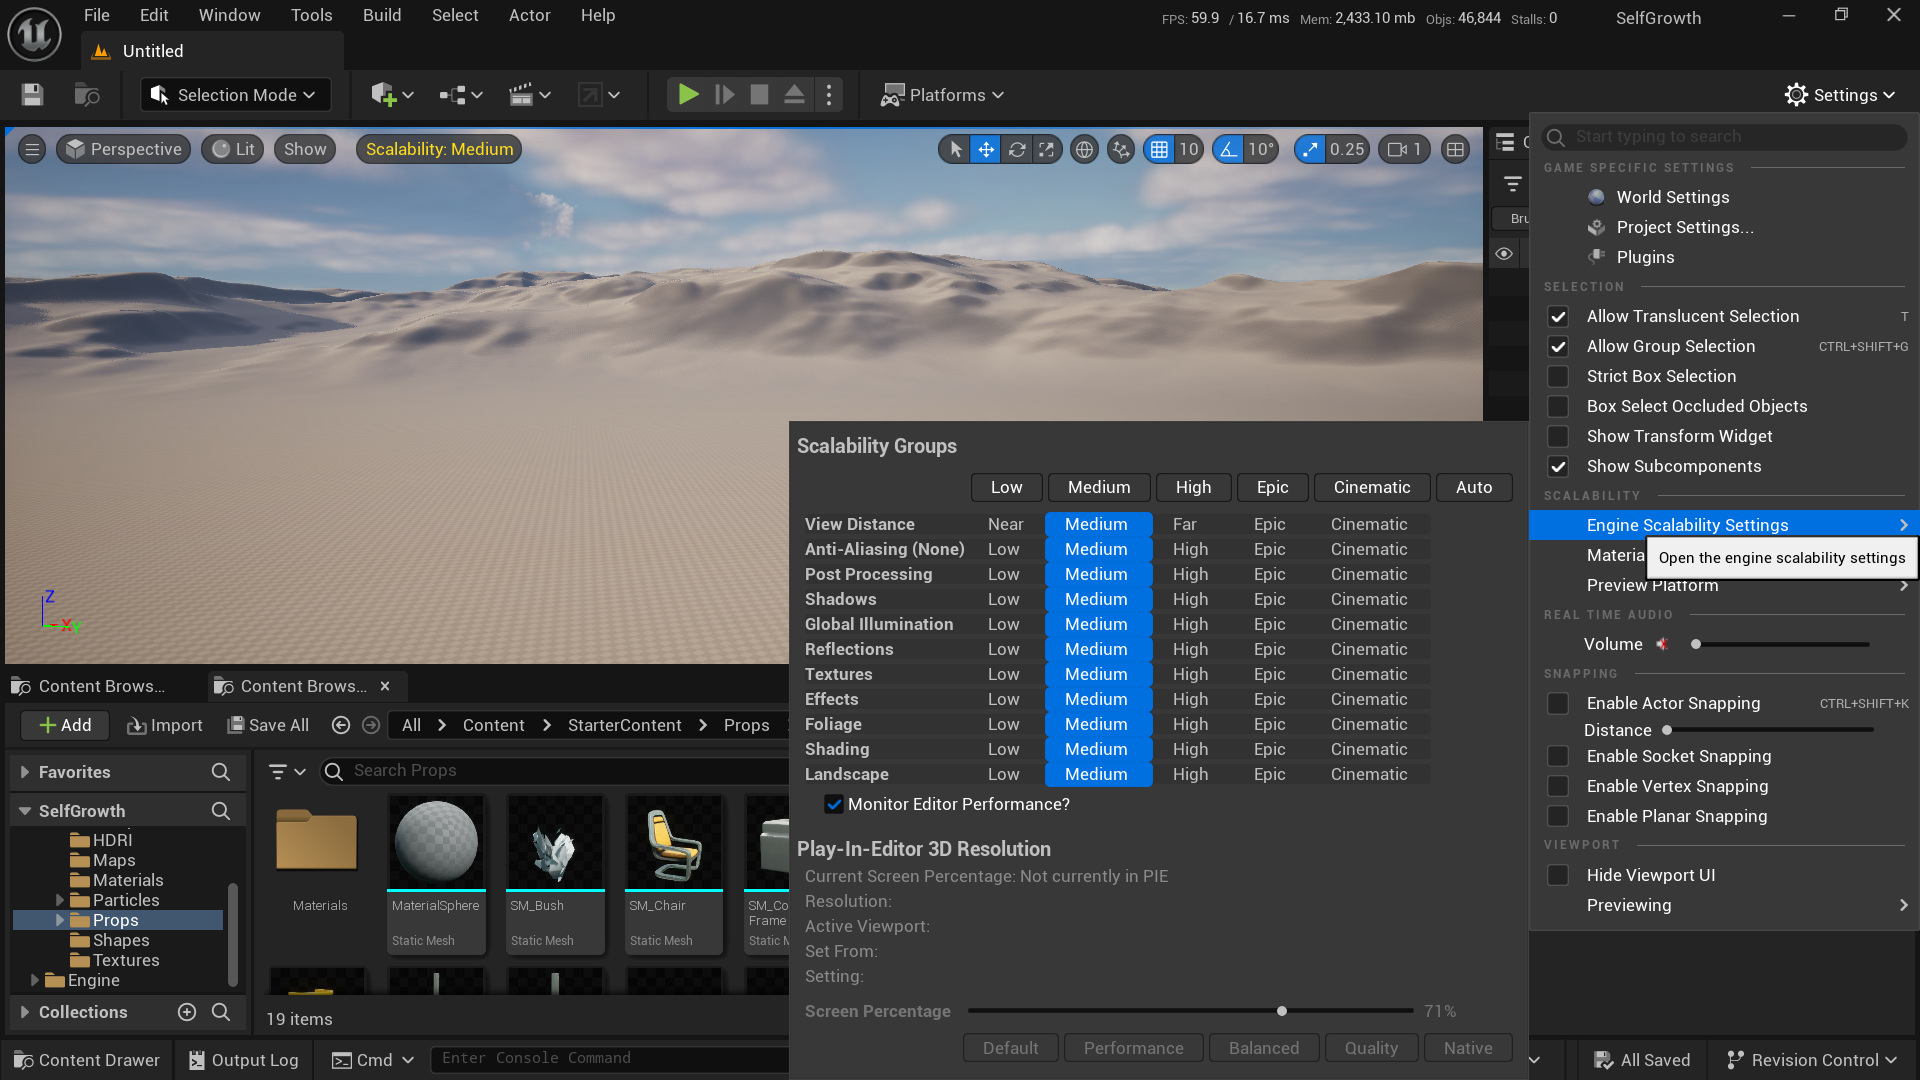
\includegraphics[width=1\textwidth]{day2images/image005.png}
    \item[Limit your FPS] In the above screenshot, find the \verb|cmd| box at the bottom. Type in \verb|t.maxfps 30| and hit enter. This will limit your FPS to 30, which tells Unreal to not try to go above 30 FPS.
    \item[Turn realtime off] There's no need to simulate grass in realtime when you don't need it (which is a very taxing operation!). You do this by pressing \verb|Conrol+R|, or, take a look in the top left corner for the three lines, and uncheck Realtime. \\[10pt]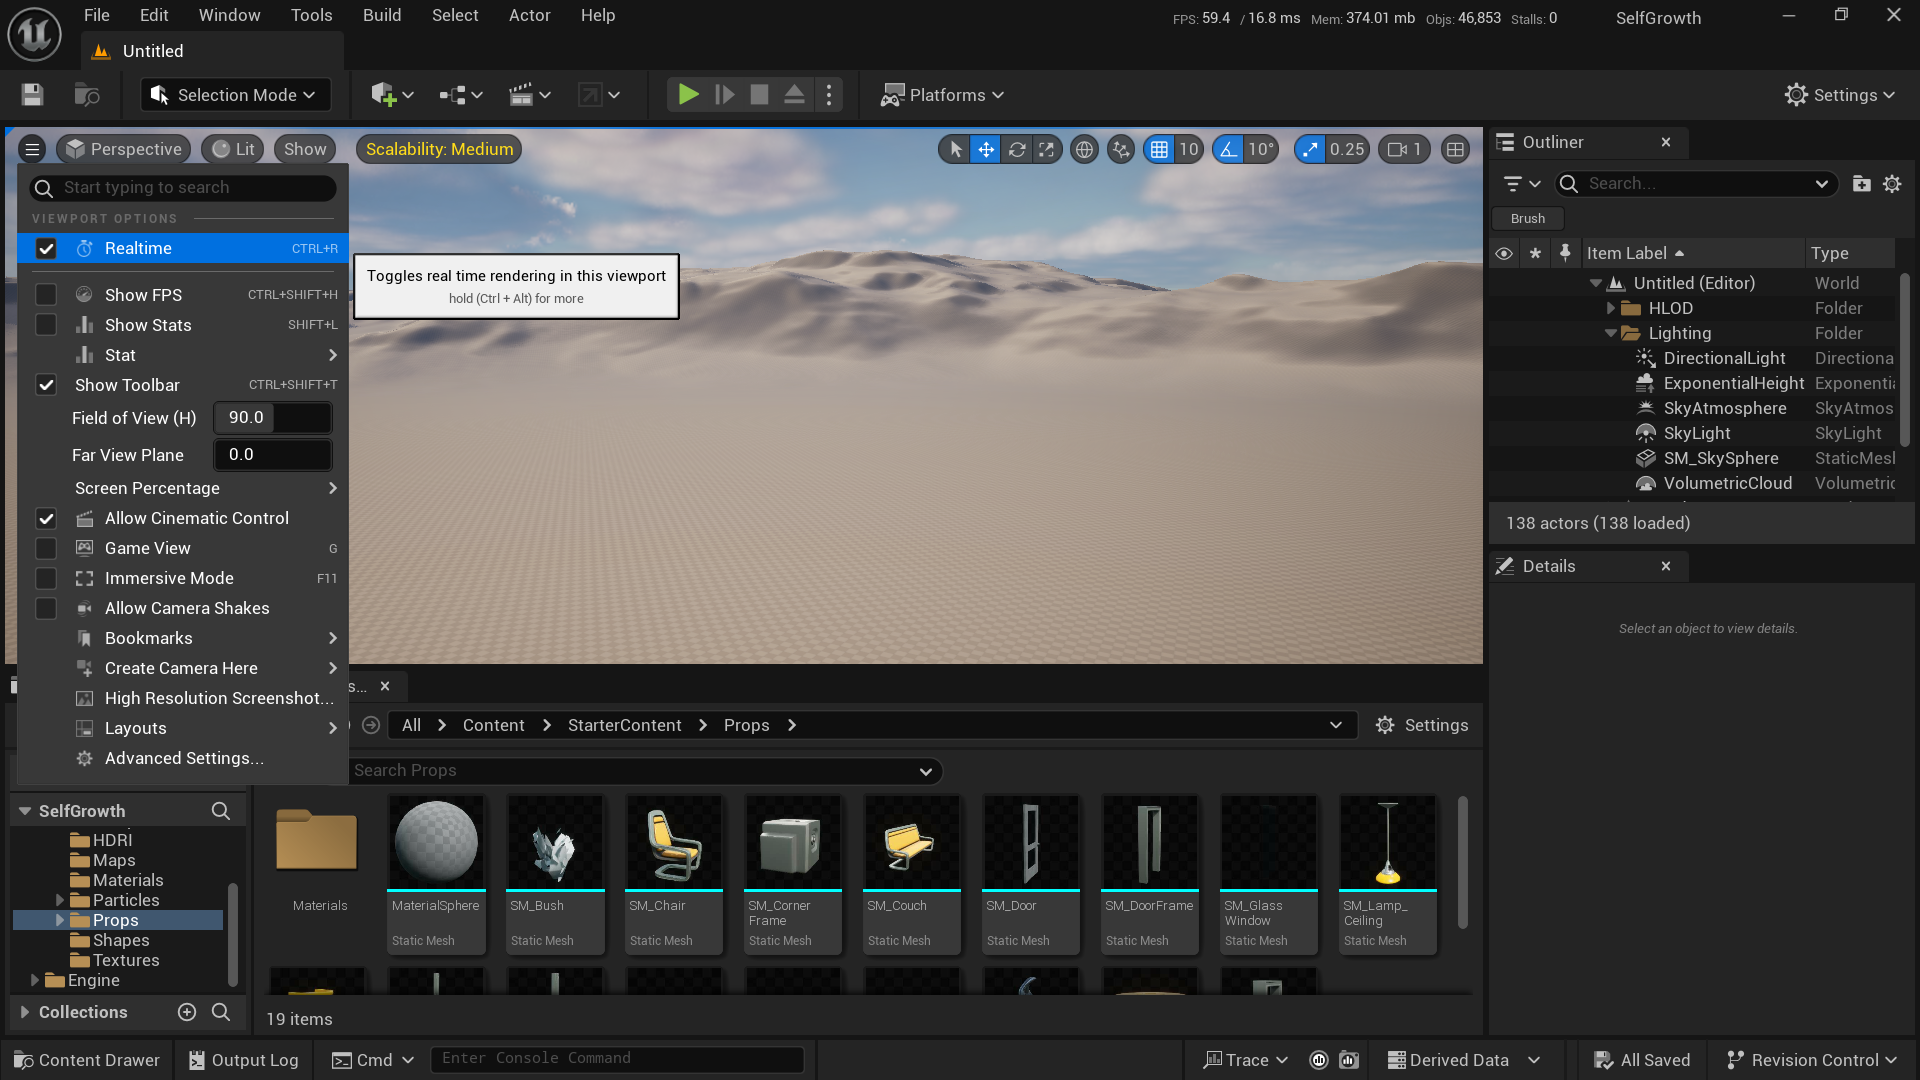
\includegraphics[width=1\textwidth]{day2images/image006.png}
    \item[Changing view modes] Being in Lit modes means you're calculating lighting, which is also expensive. You can change your mode to \emph{Unlit} for a less appealing scene but much better performant. Take a look at the button right next to \emph{Perspective}.
\end{description}

These are pretty much all the things I can think of that can help you run Unreal Engine on a slower computer. If you have any other tips, please let me know and I'll add them here. If you also have any other doubts, please let me know.




\end{document}